\documentclass[11pt]{article}
\usepackage[letterpaper,landscape,margin=0.65in]{geometry}
\usepackage{amsmath,amssymb,graphicx,booktabs,hyperref}
\hypersetup{colorlinks=true,urlcolor=blue}
\setlength{\parindent}{0pt}
\setlength{\parskip}{0.5em}
\begin{document}
\begin{center}
{\Large Guarded summation-polynomial fall degrees}\par
{\small Study report, 28 October 2026. Derived bounds and development checks; no performance claim.}
\end{center}

Let $S$ be $B$ distinct rational affine-point abscissas, $g(T)=\prod_{s\in S}(T-s)$,
and $r=x(R)$ for an affine rational target. The ordinary polynomial-ring inputs are
\[
g(x),\quad g(y),\quad g(z),\quad S_3(x,y,u),\quad S_3(u,z,r),\quad v(x-y)-1.
\]
Both point signs are allowed. The guard requires distinct first abscissas.
Every degree below is ordinary total degree with explicit membership equations.
The first-fall convention is homogeneous-top syzygies modulo Koszul syzygies.

\begin{center}
\begin{tabular}{lll}
\toprule
Setting, unsatisfiable instances & First fall & Last fall \\
\midrule
Short Weierstrass, characteristic $>3$, $B=3$ & $4$ & $5$ \\
Same model, $B\ge3$ & $B+1$ & $\max(5,B+1)\le d_F\le3B-4$ \\
Ordinary binary, $B=3$, $g(T)=T^3+c$ & $4$ & $4$ \\
Ordinary binary, $B=3$, other split cubics & $4$ & $5$ \\
Ordinary binary, $B\ge4$ & $B+1$ & $B+1\le d_F\le3B-4$ \\
\bottomrule
\end{tabular}
\end{center}

The binary curve is $Y^2+XY=X^3+a_2X^2+a_6$, $a_6\ne0$.
Its cube-orbit exception requires even extension degree, so the pair is $(4,5)$
for all three-abscissa unsatisfiable instances over $\mathbb F_{2^n}$ with odd $n$.
The bounds are mathematical derivations, not empirical fits. The growing lower
bound depends on the degree-$B$ membership input and gives no corresponding
lower bound in the variable count of a fixed-degree Boolean encoding.

\textbf{Method.} Staged multiplication and cubic reduction normalize two
quadratic fibres, then derive their scalar resultant within degree five.
Finite-grid inversion yields $1$. Characteristic two uses a Frobenius identity
instead of division by two. Closed separating superspaces give the lower bounds.
An exact triple-selector partition lifts local proofs to growing cardinality.

\textbf{Verification boundary.} Native sparse replay checks the compact historical
proof DAGs against separately supplied inputs. Native binary-field arithmetic and
the pinned cube-orbit fixture have development unit checks; no new field/base/target
sweep or timing measurement was run. Lean checks only the declarations and
hypotheses listed in \texttt{formal/PROOF\_MAP.json}. The complete filtered-closure,
grid-inversion, and elliptic-curve bridges are not formalized in this packet.

\textbf{Prior work.} The checked sources are Huang--Kosters--Yang--Yeo,
\href{https://arxiv.org/abs/1505.02532}{1505.02532}; Caminata--Gorla,
\href{https://arxiv.org/abs/2112.05579}{2112.05579}; Semaev,
\href{https://arxiv.org/abs/1504.01175}{1504.01175}; and Kosters--Yeo,
\href{https://arxiv.org/abs/1503.08001}{1503.08001}. Assumptions and repository
links are in \texttt{SOURCES.md}. No literature-priority claim is made.

\newpage
\begin{center}
{\Large Proof dependencies and unresolved transfer}\par
\vspace{0.5em}
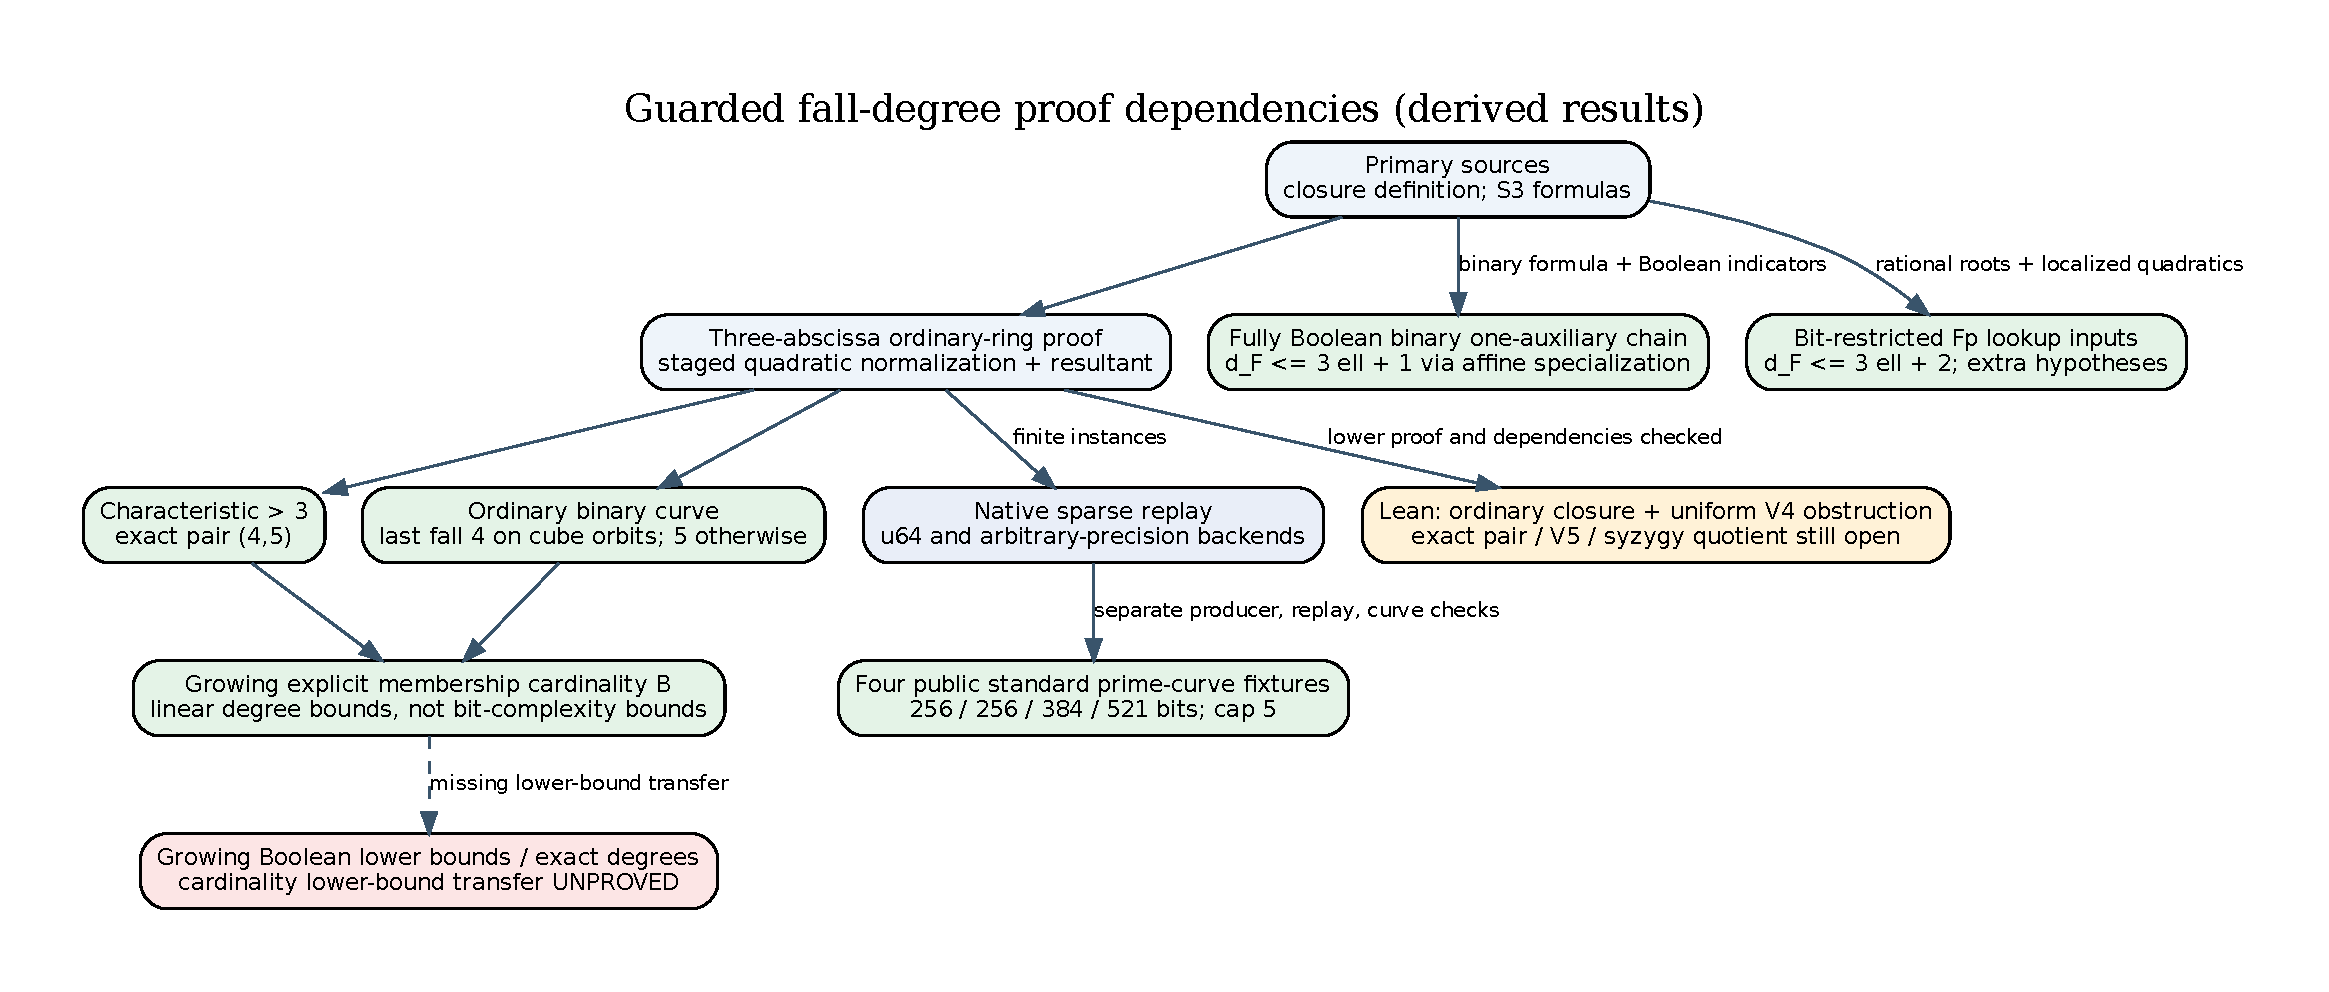
\includegraphics[width=0.99\linewidth,height=0.67\textheight,keepaspectratio]{proof-dependencies-diagram.pdf}
\end{center}

Solid arrows denote dependencies in the written arguments. The dashed arrow is
an unresolved encoding/degree transfer, not a proved implication. The Lean box
certifies algebraic identity lemmas only; native replay certifies finite proof
operations only. Neither substitutes for the complete mathematical derivation.

The existing E12 Boolean Weil-descent records are unchanged. Its completed cell
retains labels $\ge5,4,\ge5,4$, a frozen lower median of $4$, and a separate
independent closure-replay gap. The present coefficient-field theorems do not
close that gap. No cost ratio, benchmark, leaderboard or security claim follows.

\textbf{Reproducible records.} See \texttt{README.md}, the proof files,
\texttt{native/validation/}, \texttt{identities/}, and \texttt{formal/}.
The editable diagram source is \texttt{reports/proof-dependencies.dot}.
Historical Python sources are preserved as provenance, not as an execution path.
\end{document}
